%%%%%%%%%%%%%%
% Preámbulo del documento
%%%%%%%%%%%%%%
\documentclass[11pt,a4paper]{article} 
\usepackage[spanish,es-tabla,es-noindentfirst]{babel} 
\usepackage[left=2cm,right=2cm,top=2cm,bottom=2cm]{geometry} % Márgenes 
\usepackage[skip=.3\baselineskip plus 2pt,indent]{parskip} % Salto entre párrafos 
% skip= .5\baselineskip plus 2pt -> Valor por defecto

% Tipografía
\usepackage{newtxtext}
\usepackage{newtxmath}

\usepackage{marvosym,pifont,textcomp,fontawesome5}

\usepackage[T1]{fontenc} % Codificación de salida    
\usepackage[
    protrusion=true,
    activate={true,nocompatibility},
    final,
    tracking=true,
    kerning=true,
    spacing=true,
    factor=1100]{microtype}
\SetTracking{encoding={*}, shape=sc}{40}


% Generación de hiperenlaces
\usepackage[%
   pdftex,
   breaklinks,
   hidelinks=true,      % Oculta colores en los enlaces (negro)
    linktocpage=true,    % true = enlace al nº de pág., false=texto completo
%    colorlinks=true,         % true=colorea texto del enlace, false=recuadra el texto
	citecolor=red, % Color de la citas
	urlcolor=blue, % Color de las URL
	bookmarksnumbered=true % Incluye números en bookmarks
]{hyperref}
\usepackage{url}
\urlstyle{sf} % Estilo de URL sin serifas


% Listas
\usepackage{enumitem} % Mayor control de listas
\usepackage{multicol} % Elementos en varias columnas

% Tablas
\usepackage{booktabs}

% Gráficos
\usepackage{graphicx}  % Inclusión de figuras y escalado de cajas
\usepackage{float} % Control de posición de objetos flotantes y estilos
\usepackage[margin=10pt,labelfont=bf]{caption}
\captionsetup[figure]{skip=5pt} % Necesario por si se desea colocar los títulos de las figs. en la parte superior. De este modo no queda tan pegado a la figura.
\usepackage[margin=10pt,font=small,labelfont=bf]{subcaption}	% Inclusión de subfiguras
\usepackage{rotating}	% Rotación de figuras
\usepackage{pdflscape}
\usepackage{tikz}       % Librería de gráficos con comandos LaTeX

% Declaración del path donde están los archivos de figuras. 
% También se puede incluir el path en el nombre del fichero (tiene la ventaja de que TeXstudio muestra el fichero en tooltip)
\graphicspath{{../figs/}}  
\DeclareGraphicsExtensions{.pdf,.png,.jpg}
% Lista de extensiones de ficheros por orden de precedencia. De este modo no hace falta indicar la extensión del fichero y en caso de existir dos fichero con el mismos nombre y extensión diferente se emplea el que tiene una extensión con mayor prioridad.


% Con estas instrucciones se ajustan los valores del índice
\setcounter{secnumdepth}{2} % Ajusta el valor del último nivel numerado
\setcounter{tocdepth}{2} %Ajusta el valor del último nivel que aparece en TOC


\author{Jesús Salido}
\title{Inclusión avanzada de figuras en \LaTeX{}}
\date{\today}

%%%%%%%%%%%%%%
% Comienzo del documento
%%%%%%%%%%%%%%
\begin{document}

\maketitle

\begin{abstract}
	Explicación de la inclusión de figuras más complejas en documentos \LaTeX{}.
\end{abstract}

\hrule
\tableofcontents
\listoffigures
\bigskip
\hrule

\section{Gráficas matemáticas}
En muchas ocasiones es preciso recurrir a una gráfica matemática para reflejar o apoyar una idea. Existen numerosos programas que ayudan a realizar estas gráficas, en cualquiera de los casos siempre se empleará un formato vectorial (\textsf{PDF}) para incluir este tipo de figuras en nuestro documento. Nunca debe hacerse mediante una captura de pantalla pues, en este caso estaremos perdiendo mucha información al tratar como un mapa de bits algo que es un objeto matemático y, por tanto, independiente de su escala de representación.

Uno de los programas más universales para la creación de gráficas matemáticas son las hojas de cálculo como Excel. La Fig.~\ref{fig:excel} muestra un ejemplo de figura vectorial generada con ayuda de dicho programa.

\begin{figure}[hbt]
	\centering
	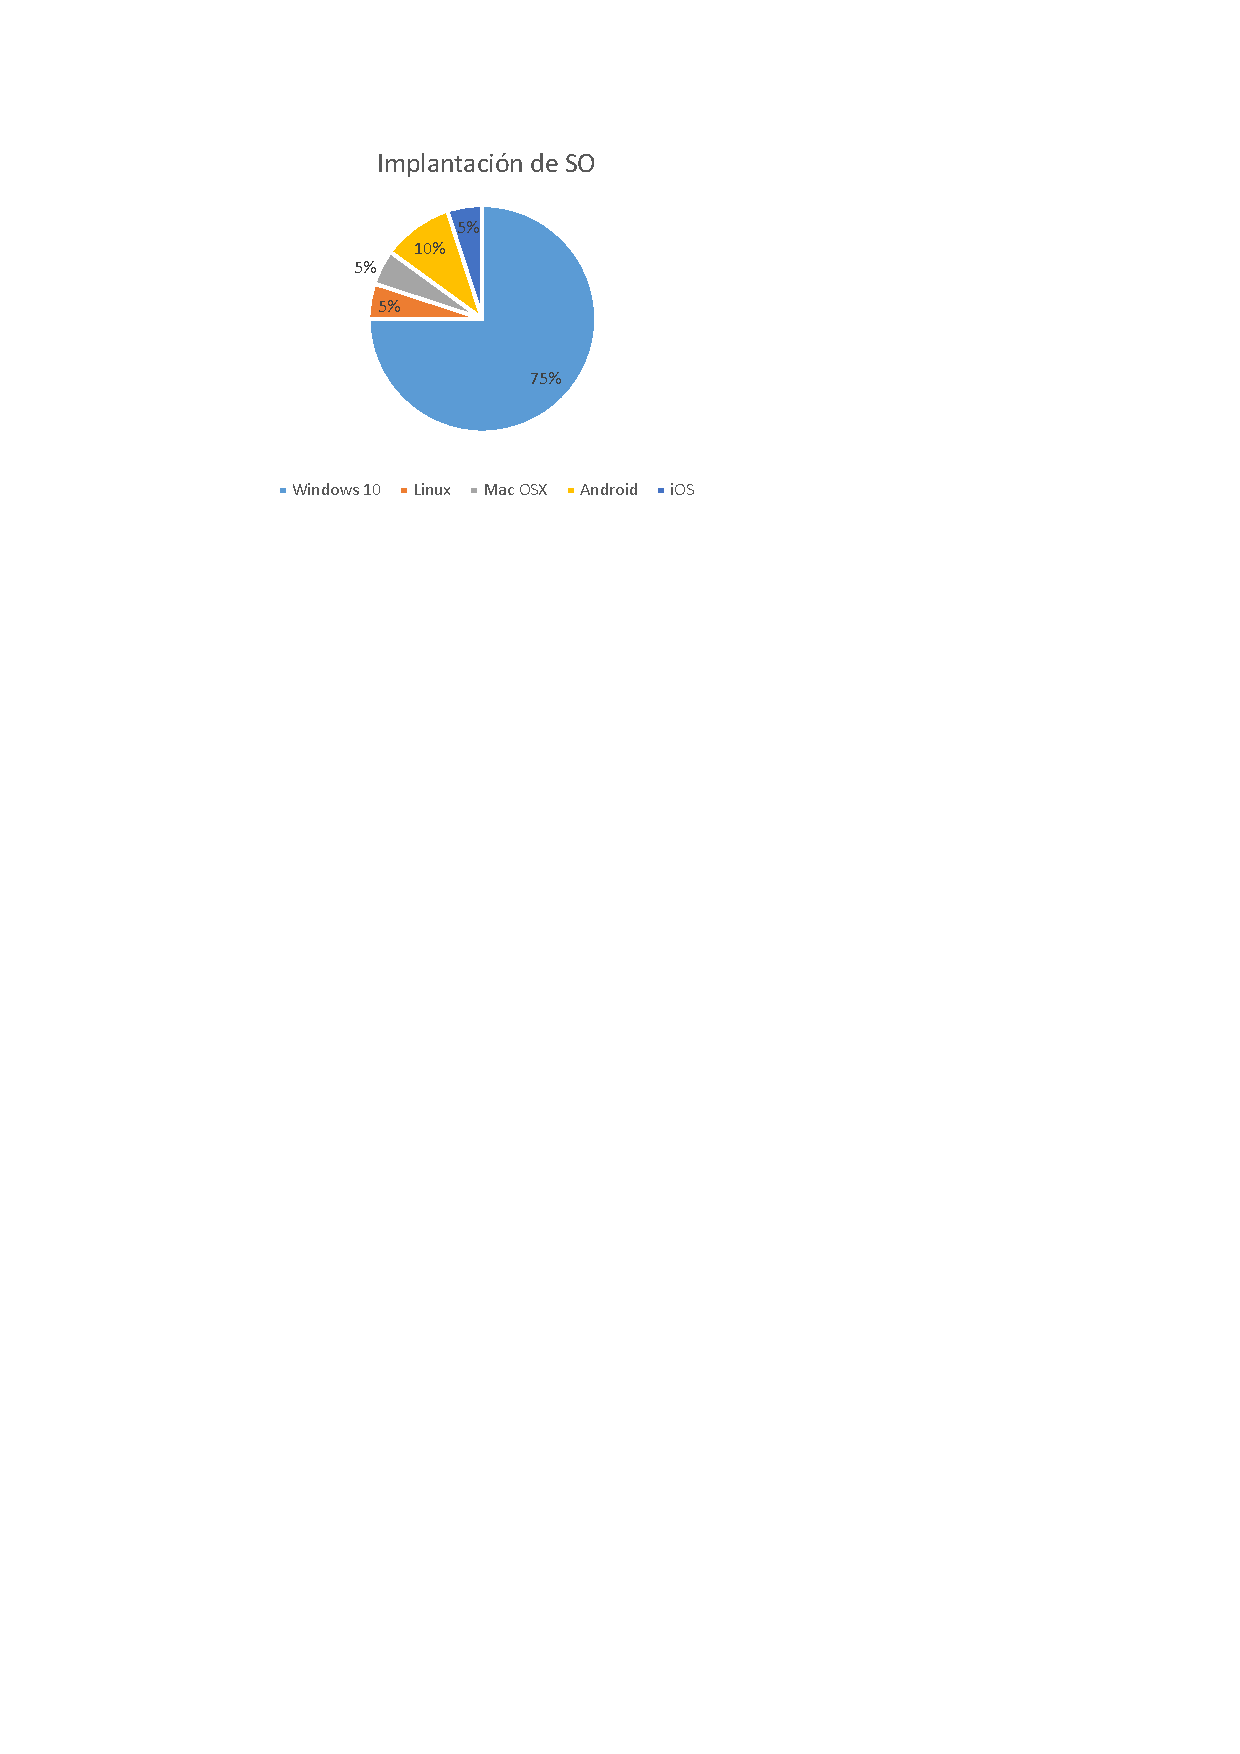
\includegraphics[width=0.5\textwidth]{../figs/EjFigsExcelOrig} 
	\caption[Gráfico de Excel]{Figura vectorial generada con Excel}
	\label{fig:excel}
\end{figure}

La Fig.~\ref{fig:matlabGrafs} muestra un ejemplo de figura vectorial generada con ayuda del programa Matlab. En este caso se observa cómo una única figura contiene distintos gráficos. La Fig.~\ref{fig:python} muestra un ejemplo de figura vectorial (\textsf{PDF}) generada con Python y la librería \textsf{Matplotlib}. En este caso se observa cómo una única figura contiene distintos gráficos, siendo este un método para crear figuras compuestas de subfiguras.

\begin{figure}[H]
	\centering
	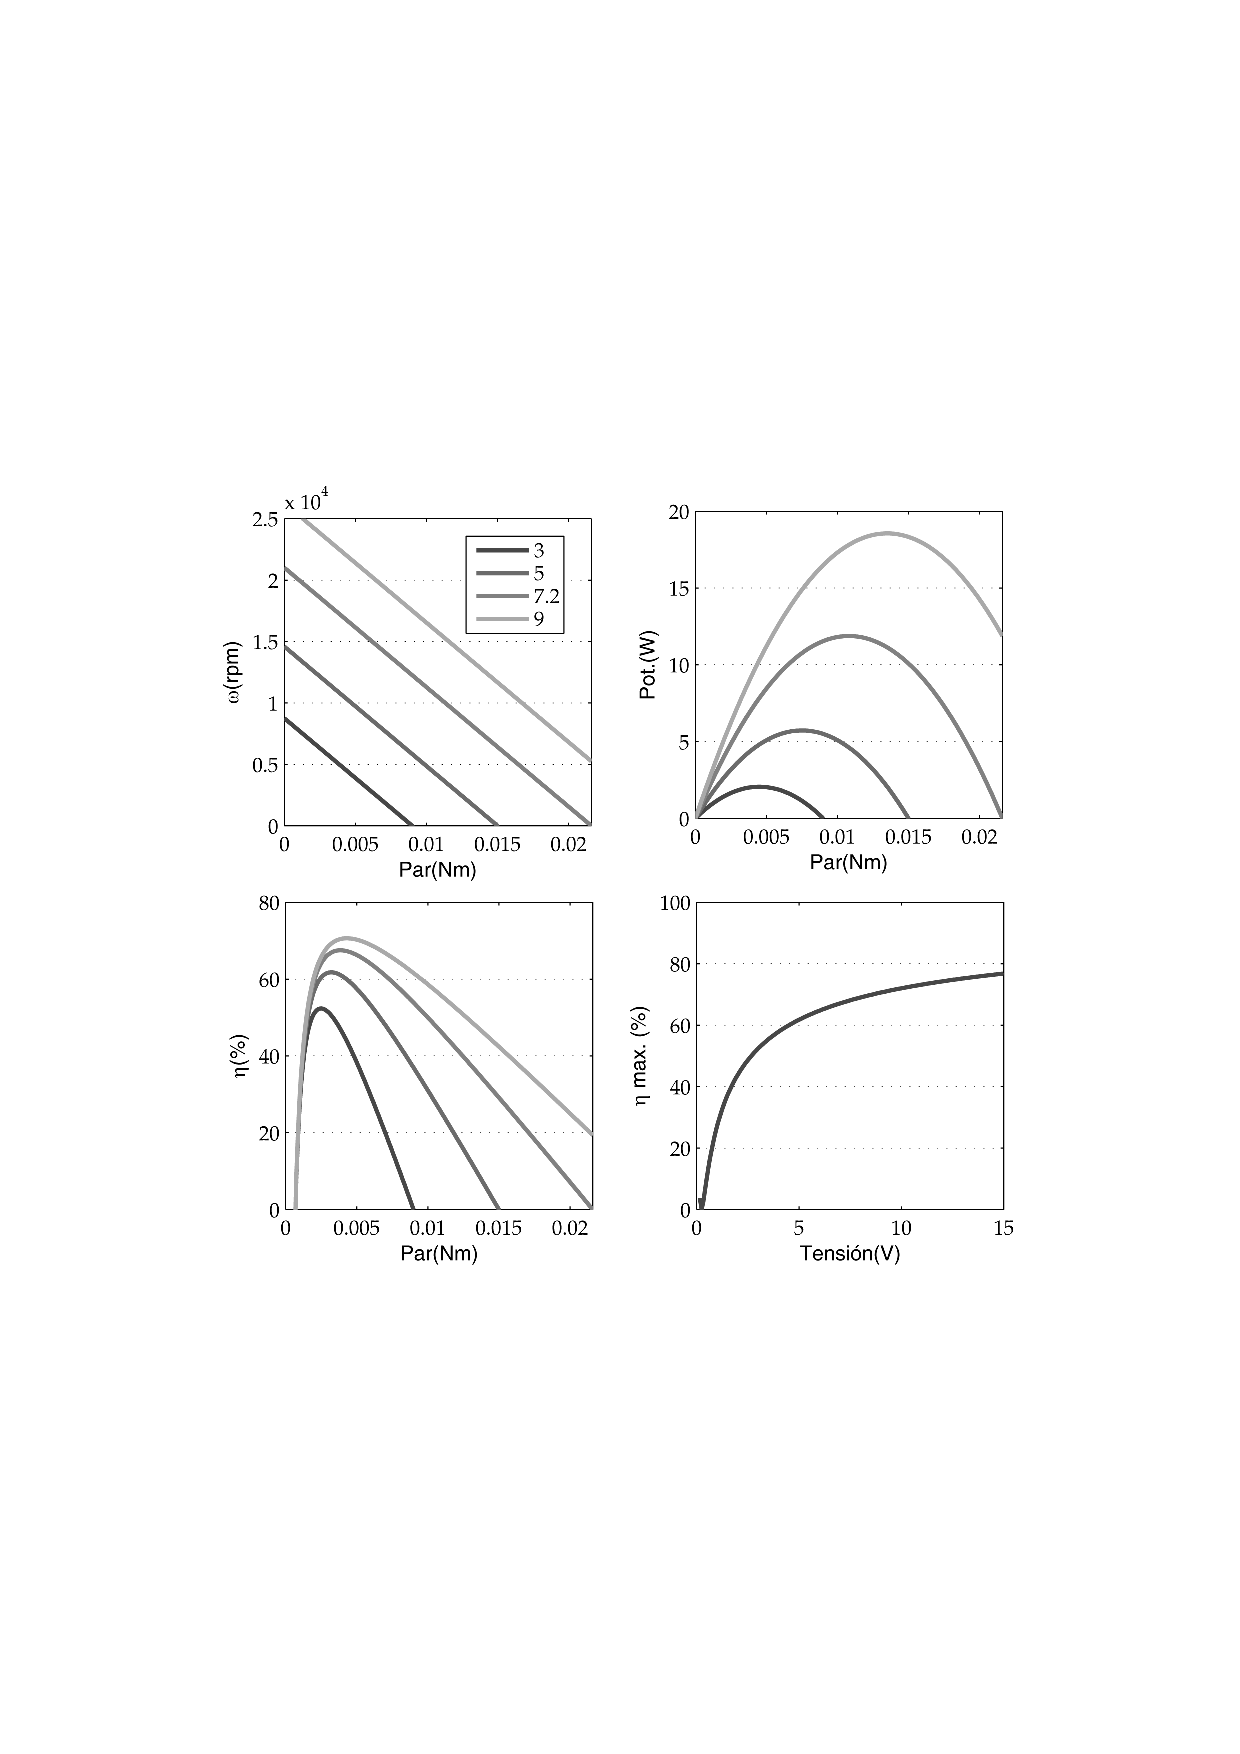
\includegraphics[width=0.8\textwidth]{../figs/matlabGrafs} 
	\caption[Gráfico de Matlab]{Figura vectorial generada con Matlab}
	\label{fig:matlabGrafs}
\end{figure}

\begin{figure}[H]
	\centering
	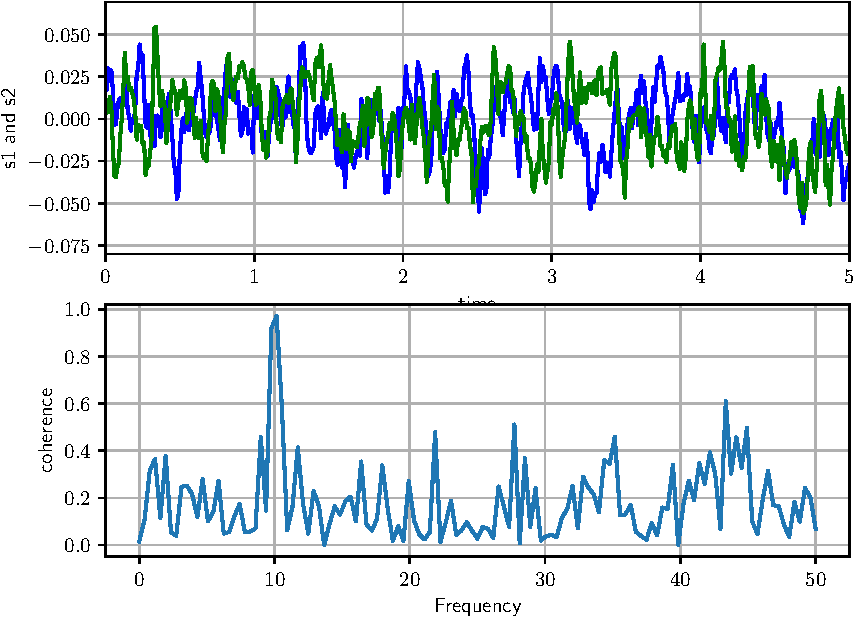
\includegraphics[width=0.8\textwidth]{../figs/fig2_py}
	\caption[Figura hecha desde Python]{Figura vectorial generada con Matplotlib (Python)}
	\label{fig:python}
\end{figure}












\section{Gráficos avanzados}
Donde se describen técnicas avanzadas de inclusión de figuras.

\subsection{Subfiguras}
La inclusión de figuras requiere al menos el empleo del paquete \texttt{graphicx} con el que ya se pueden obtener resultados muy aceptables, aunque existen otros paquetes más especializados que facilitan hacer cosas más exóticas, como el paquete \texttt{subcaption} para presentar figuras compuestas de varias subfiguras (ver ejemplos en las Figs.~\ref{fig:clock} y \ref{fig:lion}). A pesar de la posibilidad del uso del paquete \texttt{subcaption}, no se debe descartar la alternativa de la composición de subfiguras con programas externos a \LaTeX{}, e incluirlas como cualquier figura sencilla (como el proceso seguido con la Fig.~\ref{fig:2clock}). Esta alternativa hace innecesario el empleo de paquetes dedicados en \LaTeX para tal fin.

\begin{figure}[H]
	\centering
	\begin{subfigure}[b]{0.35\textwidth}
		\centering
		\includegraphics[width=\textwidth]{../figs/clockCR}
		\caption{jpg en color}\label{fig:clockCR}
	\end{subfigure}
	\begin{subfigure}[b]{0.35\textwidth}
		\centering
		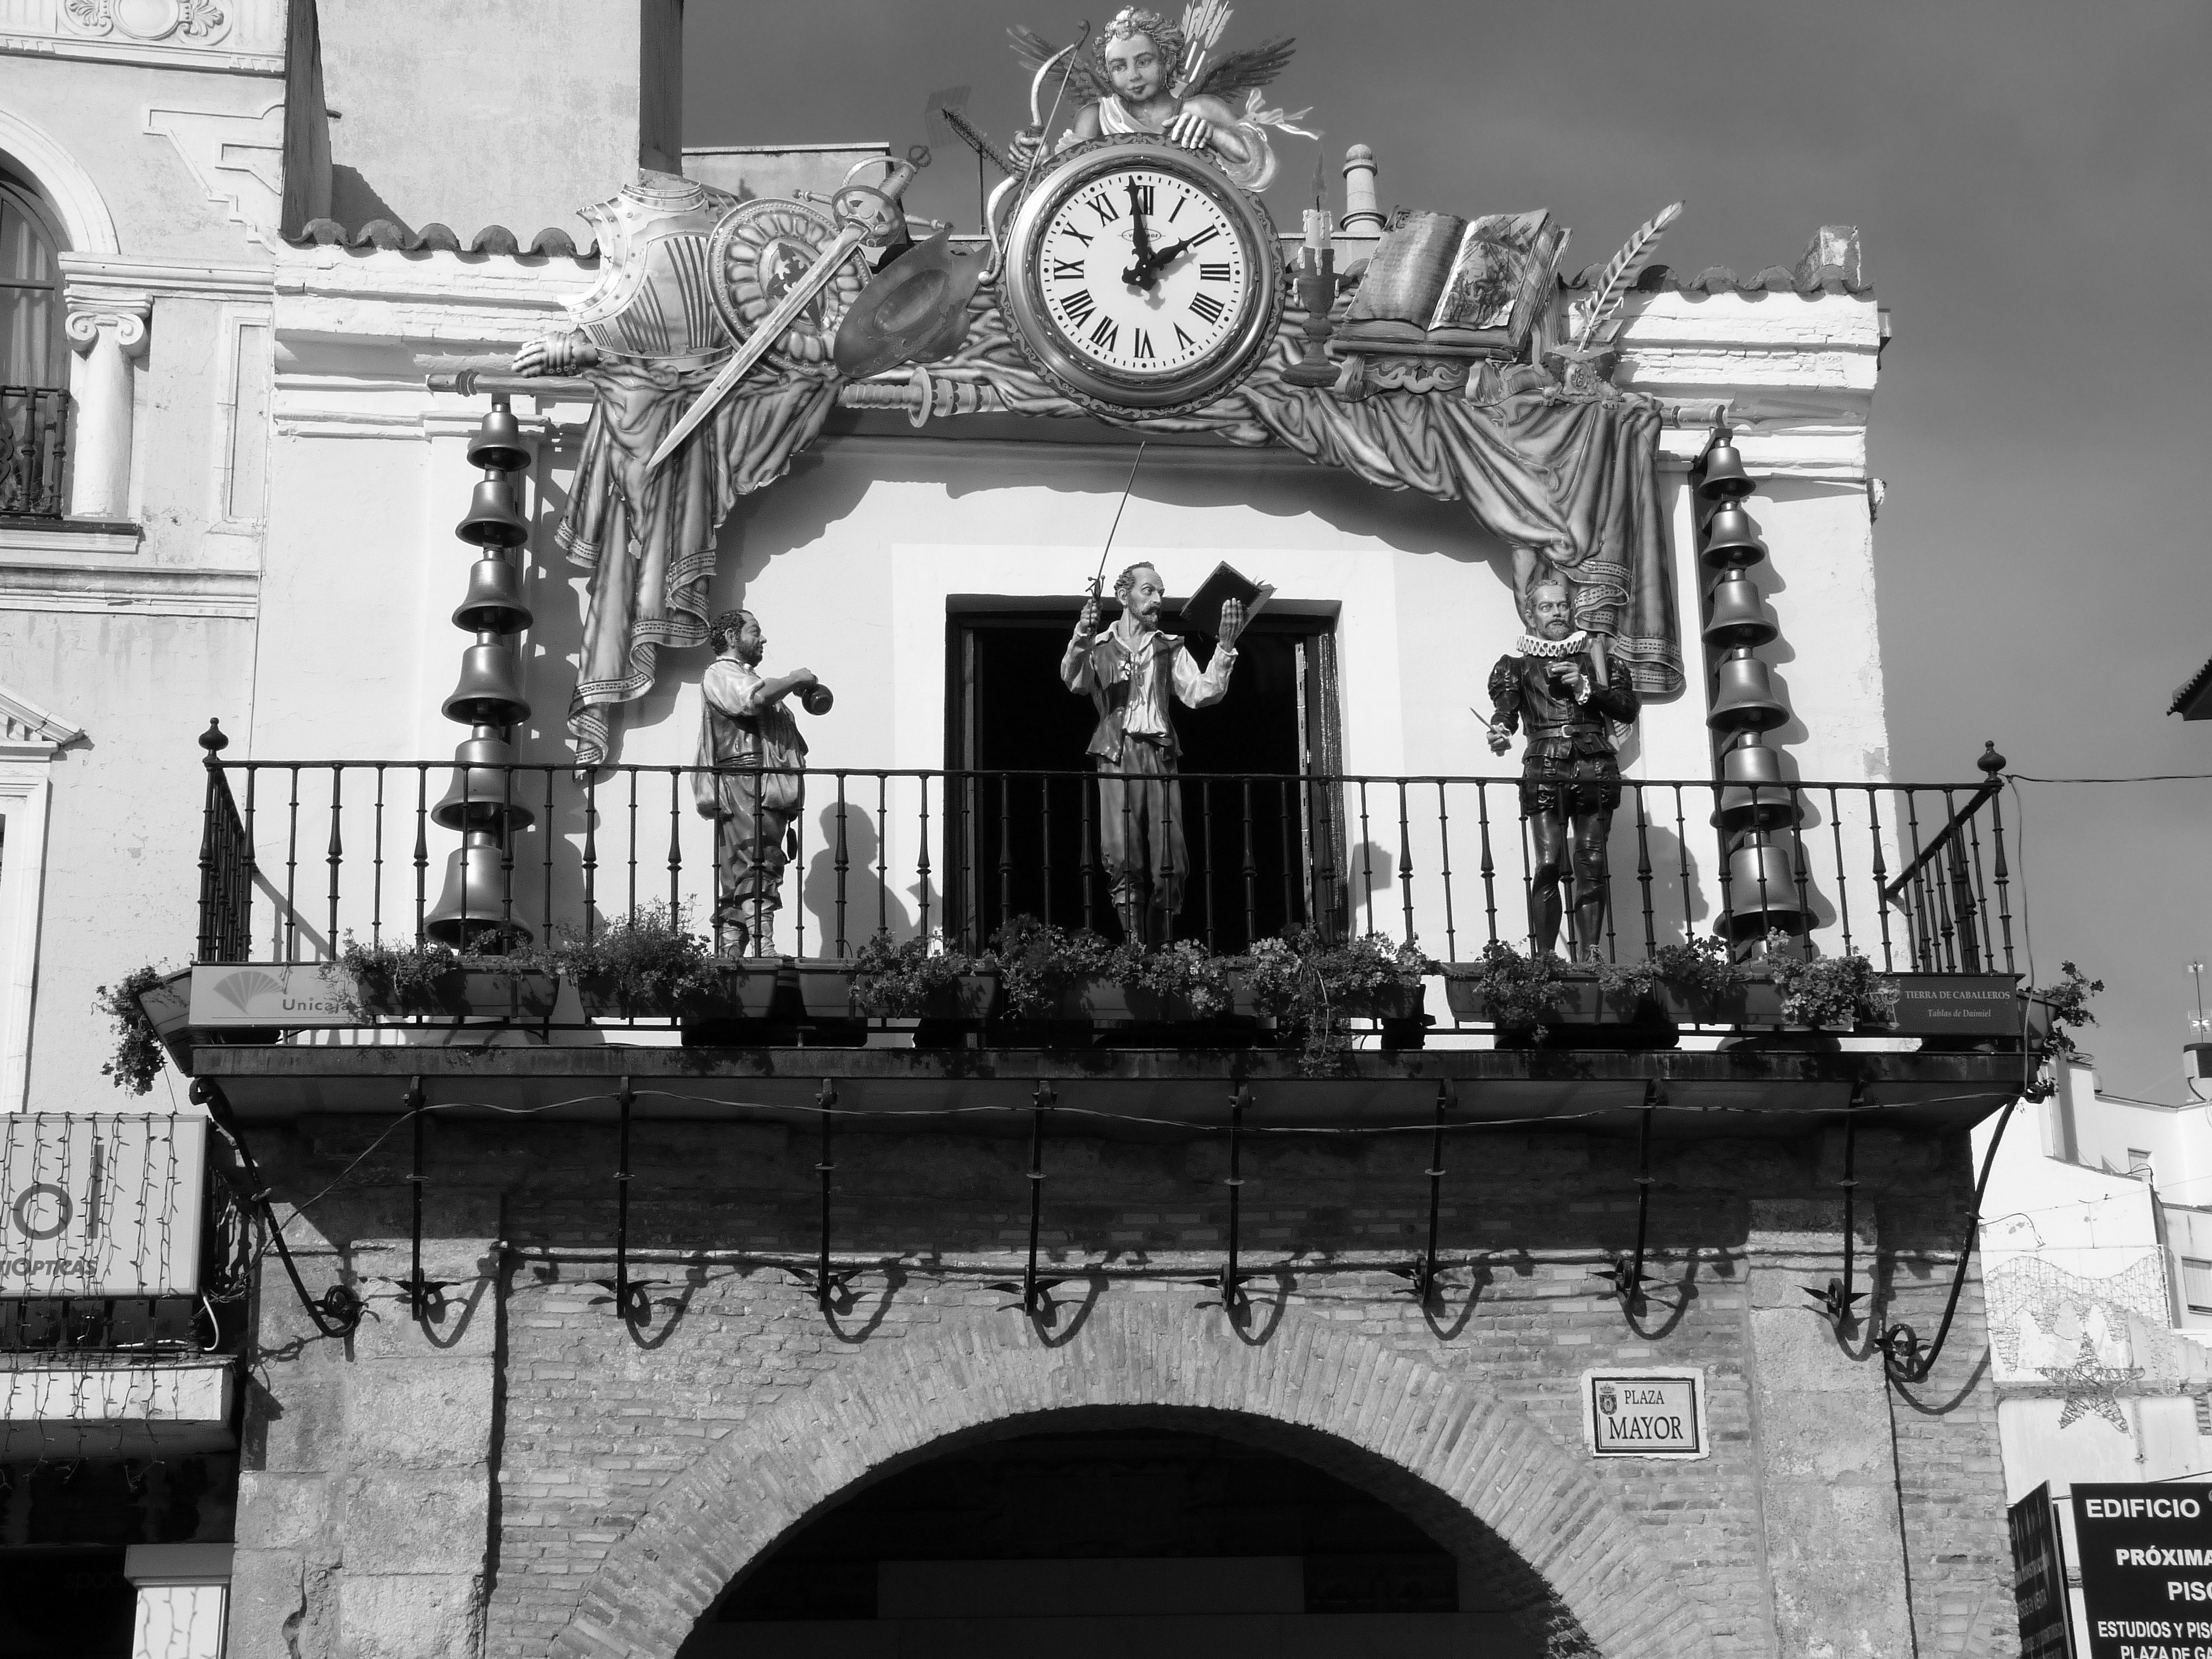
\includegraphics[width=\textwidth]{../figs/clockCRbw}
		\caption{jpg en niveles de gris}\label{fig:clockCRbw}
	\end{subfigure}
	\caption[Comparación jpg color y niveles de gris]{Ej. de paquete \texttt{subcaption} mostrando el reloj de la Plaza Mayor (Fuente: cortesía de J.~Salido)}
	\label{fig:clock}
\end{figure}

%Aquí se muestra el resultado de incluir una figura compuesta por subfiguras. Para montarlas se emplearon los programas PhotoFiltre y Powerpoint. Primero se redujo el tamaño original de las imágenes para que ocupasen menos memoria y después se montaron con Powerpoint una junto a otra dejando un espacio en blanco entre ellas. Este montaje se exporto a Photofiltre para salvarlo en el formato final.
\begin{figure}[H]
	\centering
		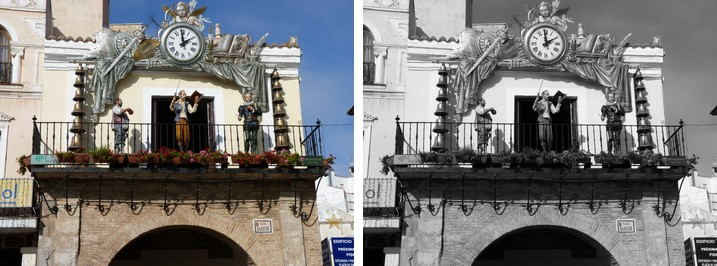
\includegraphics[width=0.7\textwidth]{../figs/2clockCR}
		\caption[Varias imágenes como una]{El reloj de la Plaza Mayor en color (izda.) y niveles de gris (dcha.)}
	\label{fig:2clock}
\end{figure}

Siempre que se tenga un fichero de imagen (mapa de bits) con un fondo blanco u otro color plano, debería intentarse transformar en una imagen con fondo transparente convirtiéndola al formato \texttt{.png} (véase ejemplo en la Fig.~\ref{fig:lion}).

\begin{figure}[H]
	\centering
  	\begin{subfigure}[b]{0.4\textwidth}
  		\centering
		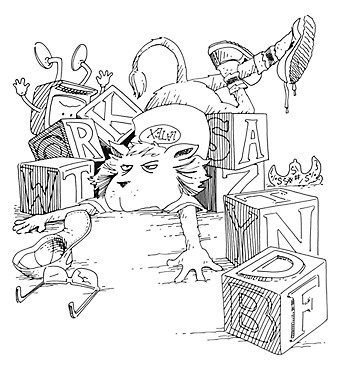
\includegraphics[width=0.8\textwidth]{../figs/lionL.jpg}
		\caption{jpg}\label{fig:lionLjpg}
  	\end{subfigure}
  	\begin{subfigure}[b]{0.4\textwidth}
  		\centering
		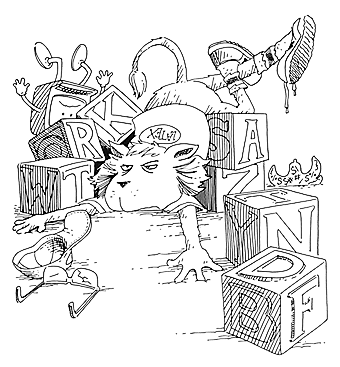
\includegraphics[width=0.8\textwidth]{../figs/lionL.png}
		\caption{png con fondo transparente}\label{fig:lionpng}
  	\end{subfigure}
  	\caption[Comparación jpg y png con transparencia]{Comparativa de formatos bitmap (cortesía de D.~Wright)}
	\label{fig:lion}
\end{figure}

Si se desea, es posible usar imágenes en color. Esto es muy conveniente para documentos electrónicos que se van a visualizar en la pantalla de un computador. Sin embargo, para documentos que serán impresos hay que considerar si la impresión se realizará a color o en niveles de gris para que el resultado final mantenga una legibilidad adecuada. 

En la Fig.~\ref{fig:escudo} se comparan los resultados obtenidos cuando la figura se inserta en formato vectorial (escalable) y cuando se hace como mapa de bits (no escalable). En este ejemplo se muestran dos versiones para el escudo de la Ingeniería Informática (cortesía de CRySoL).\footnote{El escudo basado en el núcleo de ferrita que acompaña la distribución de este documento ha sido realizado por Francisco Moya, David Villa e Ignacio Díez y su inclusión en el documento final debe respetar los derechos de la licencia CC BY-SA 3.0 con la que se distribuye.}

\begin{figure}[H]
	\centering
	\begin{subfigure}[b]{0.3\textwidth}
		\centering
		
\includegraphics[width=0.7\textwidth]{../figs/escudoInfBW.pdf}
		\caption{Gráfico vectorial \textsf{PDF}}\label{fig:escudoPDF}
	\end{subfigure}
	\begin{subfigure}[b]{0.3\textwidth}
		\centering
		
\includegraphics[width=0.7\textwidth]{../figs/escudoInfBW.png}
		\caption{Gráfico png}\label{fig:escudoPNG}
	\end{subfigure}
	\caption[Comparación \textsf{PDF} y png]{Comparando distintos formatos para el escudo de Informática (cortesía de CRySoL).}
	\label{fig:escudo}
\end{figure}











\subsection{Imágenes con elementos vectoriales}
En ocasiones es necesario recurrir a capturas de pantalla sobre las que es preciso realizar alguna anotación gráfica, por ejemplo añadiendo flechas y bloques de texto. Este es un caso que puede aparecer cuando se explica el funcionamiento de un programa informático (p.~ej., en un manual). La captura siempre se debe llevar a cabo al mayor tamaño posible sobre la pantalla y se debe salvar en formato \texttt{.png}. Generalmente, las herramientas de captura permiten la edición de la captura añadiéndole elementos gráficos e incluso texto. En este caso los elementos añadidos 
forman parte del fichero \texttt{.png} y, por tanto, son definidos como mapa de bits. Si se desea mantener las características escalables de los elementos gráficos, éstos se deben añadir mediante algún programa de edición vectorial (p.~ej.,  
\textsf{Inkscape}, \textsf{LibreOffice Draw}, \textsf{Dia}, \textsf{Visio}, etc.) y salvar el fichero resultante en formato \texttt{.pdf}. Las figs.~\ref{fig:texmk02} y \ref{fig:texmk03} muestran la diferencia del resultado final.

\begin{figure}[H]
	\centering
	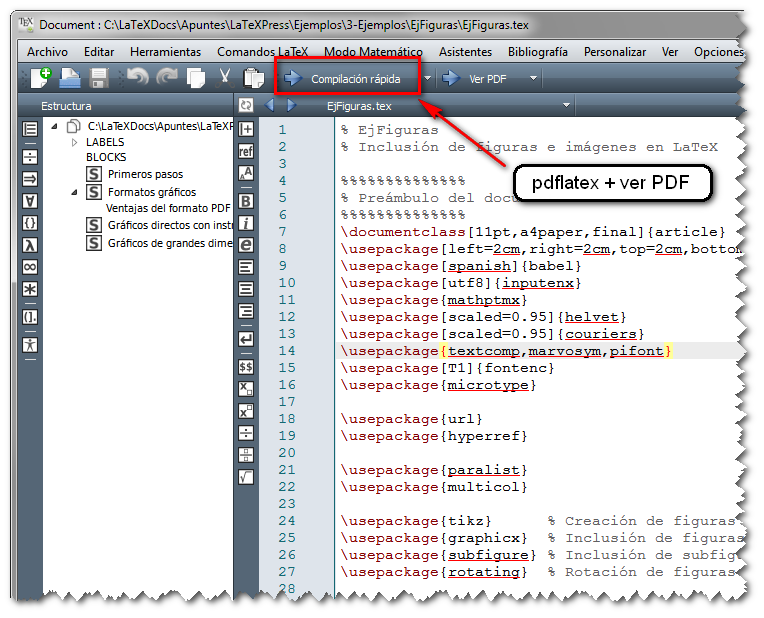
\includegraphics[width=0.6\textwidth]{../figs/texmk02} 
	\caption[Captura con gráfico en \texttt{png}]{Captura de pantalla con añadido gráfico en formato \texttt{png}}
	\label{fig:texmk02}
\end{figure}

\begin{figure}[H]
	\centering
	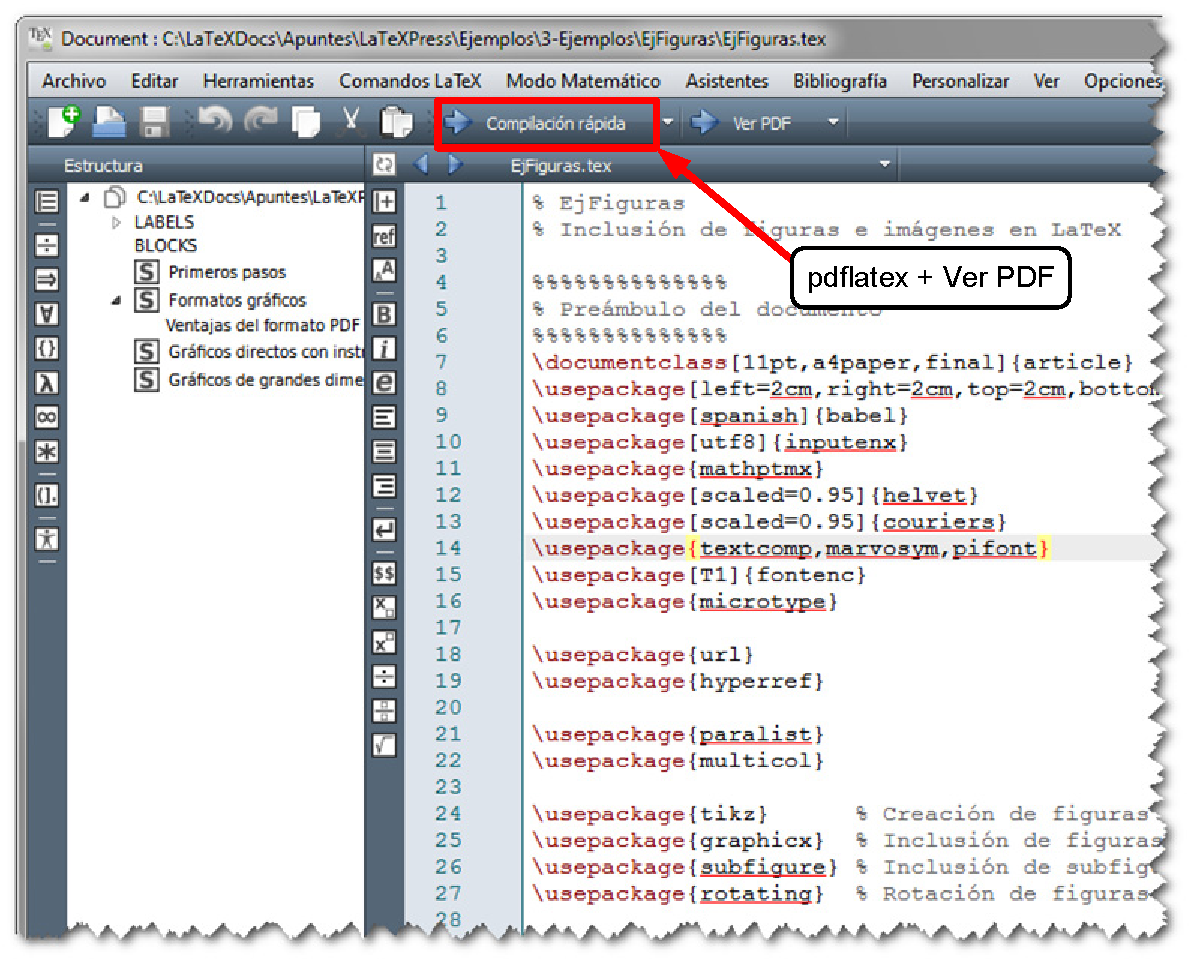
\includegraphics[width=0.6\textwidth]{../figs/texmk03} 
	\caption[Captura con gráfico en \texttt{pdf}]{Captura de pantalla con añadido gráfico en formato \texttt{pdf}}
	\label{fig:texmk03}
\end{figure}











\subsection{Inclusión de páginas individuales de un \textsf{PDF} multipágina}
La Fig.~\ref{fig:visio_mp} nos muestra el procedimiento para usar los ficheros \textsf{PDF} multipágina al incluir el gráfico de una página concreta.

\begin{figure}[H]
	\centering
	\includegraphics[page=2,width=0.5\textwidth]{../figs/visio_mp} 
	\caption[Gráfico de Visio multipágina]{Figura vectorial generada con Microsoft Visio en un fichero multipágina}
	\label{fig:visio_mp}
\end{figure}













\subsection{Gráficos directos con instrucciones \TeX}
Además de los aspectos comentados aquí sobre la inclusión de imágenes y gráficos, \LaTeX{} dispone de una infinidad de recursos que pueden por sí mismo ser objeto de un curso. Un paquete muy poderoso para generar gráficos con instrucciones \LaTeX{} es \texttt{tikz} (ver Fig.~\ref{fig:tikz}). La cantidad y variedad de gráficos que se puede realizar es muy numerosa\footnote{Muchos ejemplos de uso en \url{http://www.texample.net/tikz/examples/}, \url{https://tikz.net/} y \url{https://www.overleaf.com/gallery/tagged/tikz/}.} aunque su uso requiere un conocimiento muy profundo y no es apropiado para principiantes.

\begin{figure}[H]
	\centering
	{\shorthandoff{>}
        \begin{tikzpicture}[scale=0.2]
        \tikzstyle{every node}+=[inner sep=0pt]
        \draw [black] (9.6,-8.7) circle (3);
        \draw (9.6,-8.7) node {$Q_0/0$};
        \draw [black] (9.6,-8.7) circle (2.4);
        \draw [black] (35,-7.9) circle (3);
        \draw (35,-7.9) node {$Q_1/1$};
        \draw [black] (35,-25.6) circle (3);
        \draw (35,-25.6) node {$Q_3/1$};
        \draw [black] (9.6,-25.6) circle (3);
        \draw (9.6,-25.6) node {$Q_2/0$};
        \draw [black] (9.6,-3.5) -- (9.6,-5.7);
        \draw (9.6,-3) node [above] {$INIT/CLR$};
        \fill [black] (9.6,-5.7) -- (10.1,-4.9) -- (9.1,-4.9);
        \draw [black] (6.782,-9.696) arc (317.19637:29.19637:2.25);
        \draw (2.23,-7.78) node [left] {$00$};
        \fill [black] (7.1,-7.07) -- (6.85,-6.16) -- (6.17,-6.89);
        \draw [black] (11.787,-6.652) arc (128.24239:55.3656:17.604);
        \fill [black] (32.69,-5.99) -- (32.31,-5.13) -- (31.75,-5.95);
        \draw (22.1,-2.34) node [above] {$01$};
        \draw [black] (35.376,-4.935) arc (200.49955:-87.50045:2.25);
        \draw (40.23,-1.77) node [above] {$10$};
        \fill [black] (37.58,-6.4) -- (38.51,-6.58) -- (38.16,-5.65);
        \draw [black] (37.962,-7.506) arc (125.31508:-162.68492:2.25);
        \draw (42.16,-10.78) node [right] {$01$};
        \fill [black] (37.11,-10.01) -- (37.17,-10.95) -- (37.99,-10.38);
        \draw [black] (12.482,-7.87) arc (104.17982:79.42817:45.722);
        \fill [black] (32.07,-7.25) -- (31.38,-6.61) -- (31.19,-7.6);
        \draw (22.21,-5.95) node [above] {$10$};
        \draw [black] (32.154,-8.847) arc (-73.76473:-102.62728:39.452);
        \fill [black] (12.5,-9.47) -- (13.17,-10.13) -- (13.39,-9.15);
        \draw (22.4,-10.95) node [below] {$00$};
        \draw [black] (37.808,-24.577) arc (137.74177:-150.25823:2.25);
        \draw (42.36,-26.44) node [right] {$11$};
        \fill [black] (37.52,-27.21) -- (37.78,-28.11) -- (38.45,-27.37);
        \draw [black] (35.751,-10.803) arc (11.59172:-11.59172:29.595);
        \fill [black] (35.75,-10.8) -- (35.42,-11.69) -- (36.4,-11.49);
        \draw (36.85,-16.75) node [right] {$00$};
        \draw [black] (8.855,-22.695) arc (-168.66522:-191.33478:28.215);
        \fill [black] (8.86,-22.7) -- (9.19,-21.81) -- (8.21,-22.01);
        \draw (7.8,-17.15) node [left] {$11$};
        \draw [black] (6.92,-26.923) arc (324:36:2.25);
        \draw (2.35,-25.6) node [left] {$10$};
        \fill [black] (6.92,-24.28) -- (6.57,-23.4) -- (5.98,-24.21);
        \draw [black] (10.124,-28.542) arc (37.82895:-250.17105:2.25);
        \draw (6.5,-32.66) node [below] {$01$};
        \fill [black] (7.58,-27.81) -- (6.64,-27.9) -- (7.26,-28.69);
        \draw [black] (11.64,-23.401) arc (135.83658:113.90487:65.965);
        \fill [black] (32.23,-9.05) -- (31.3,-8.92) -- (31.7,-9.83);
        \draw (19.74,-14.74) node [above] {$00$};
        \draw [black] (33.038,-10.169) arc (-42.35986:-67.89868:56.882);
        \fill [black] (12.41,-24.55) -- (13.34,-24.71) -- (12.96,-23.78);
        \draw (24.99,-19.01) node [below] {$11$};
        \draw [black] (12.535,-24.98) arc (100.34158:79.65842:54.397);
        \fill [black] (32.07,-24.98) -- (31.37,-24.34) -- (31.19,-25.33);
        \draw (22.3,-23.6) node [above] {$11$};
        \draw [black] (32.093,-26.339) arc (-77.62637:-102.37363:45.7);
        \fill [black] (12.51,-26.34) -- (13.18,-27) -- (13.4,-26.02);
        \draw (22.3,-27.9) node [below] {$10$};
        \draw [black] (32.845,-27.681) arc (-51.12017:-128.87983:16.799);
        \fill [black] (11.76,-27.68) -- (12.06,-28.57) -- (12.69,-27.79);
        \draw (22.3,-31.9) node [below] {$01$};
        \end{tikzpicture}
	}
	\caption[Ejemplo de gráfico con Ti\textit{K}Z]{Figura realizada con paquete \texttt{tikz} para un diagrama de transición de estados correspondiente a un autómata de Moore}\label{fig:tikz}
\end{figure}









\subsection{Gráficos de grandes dimensiones}
Cuando se presenta la necesidad de incluir un gráfico demasiado grande para el tamaño de la página, una opción muy apropiada es la impresión del gráfico en modo girado en una página aparte. Este efecto se consigue con el entorno \texttt{sidewaysfigure} proporcionado por el paquete \texttt{rotating}. La Fig.~\ref{fig:girada} muestra un ejemplo del entorno citado con un gráfico \textsf{PDF}.

\begin{sidewaysfigure}
	\centering
	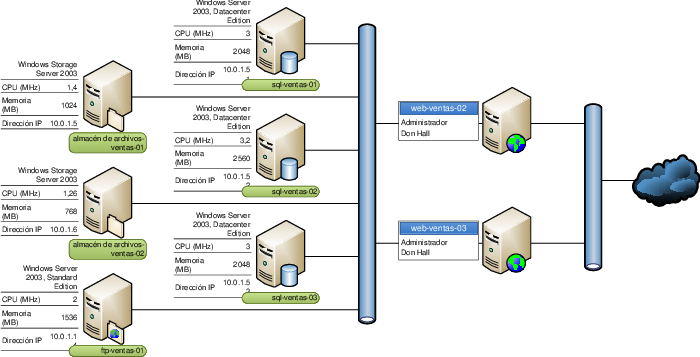
\includegraphics[width=0.98\textheight]{../figs/network} 
	\caption[Gráfico girado de Visio]{Figura vectorial con impresión girada}
	\label{fig:girada}
\end{sidewaysfigure}


% Página en formato apaisado
\begin{landscape}
También es posible imprimir una página en formato apaisado cuando contiene una figura muy ancha. Este efecto se consigue con el paquete \texttt{pdflscape} y el entorno \texttt{landscape} proporcionado. La figura~\ref{fig:apaisada} muestra un ejemplo de figura en página apaisada.
\begin{figure}[H]
	\centering
	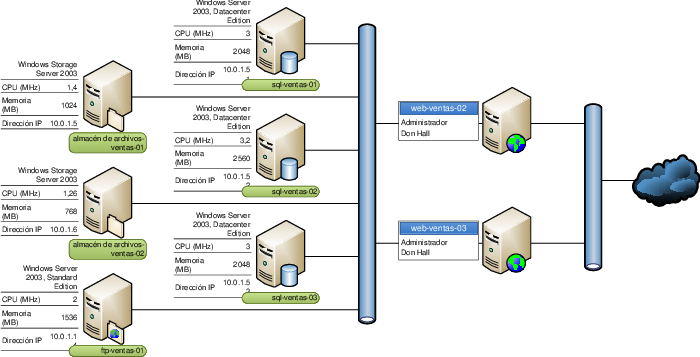
\includegraphics[width=0.98\linewidth]{../figs/network} 
	\caption[Gráfico apaisado de Visio]{Figura vectorial con vista e página apaisada}
	\label{fig:apaisada}
\end{figure}
\end{landscape}

\end{document}